\documentclass[10pt]{article}
\usepackage{icmlko}

\icmlmeta{IP 파운데이션 월드모델}{74}{가장 잘 맞히는 도메인이 가장 못 가르쳤다}{여덟째 도메인이 상충 법칙을 $r=+0.998$까지 밀어붙였다 --- 그리고 닮은 도메인이 서로에게 특별하지 않다}

\begin{document}

\twocolumn[
\icmlheader

\begin{abstract}
여덟째 도메인을 넣었다 --- \textbf{모바일 게임 1,991건}(앱스토어 인기 차트,
키 불필요). 축 배선을 스팀 게임과 \emph{일부러 같게} 맞췄다(언어 수 · 개발사
이력 · 가격 · 앱 용량). 결과가 셋이다. \textbf{첫째, 판정치가 크게 올랐다} ---
앙상블 $\rho$가 $+$0.2744에서 \textbf{$+$0.3235}로, 구간 반폭이 0.0453에서
0.0431로. \textbf{둘째, 모바일이 역대 최고 도메인이다} --- 자기 $\rho$ $+$0.656,
대상으로 $+$0.467 둘 다 1위. \textbf{그런데 출처로는 $+$0.251이고
모바일$\to$팝업은 $+$0.223으로 나머지 평균($+$0.434)보다 \emph{0.211 낮다}.}
노트 38 · 40의 상충 법칙이 여기서 완성된다 --- 애니를 뺀 일곱 점에서 자기
$\rho$와 대상 전이의 상관이 \textbf{$r=+0.998$}, 출처 전이와는 $-$0.707이다.
\textbf{셋째, 닮은 것이 특별하지 않다.} 모바일과 스팀 게임은 표면이 거의 같은데
게임$\to$모바일이 나머지보다 $+$0.052 나을 뿐이고 모바일$\to$게임은 오히려
$-$0.023이다. 그리고 방향은 \textbf{안 뒤집혔다} --- 애니가 여전히 유일한
사례다. 합의 정향은 여덟 도메인에서도 애니를 정확히 지목하지만 이득이 0이
됐고($-$0.0003), 게이트는 이제 안 무너지지만($+$0.3234) 균등($+$0.3235)과
같다. \textbf{합치는 것 위로 더 얹을 것이 아직 없다.}
\end{abstract}
]

\begin{figure*}[t]
\centering
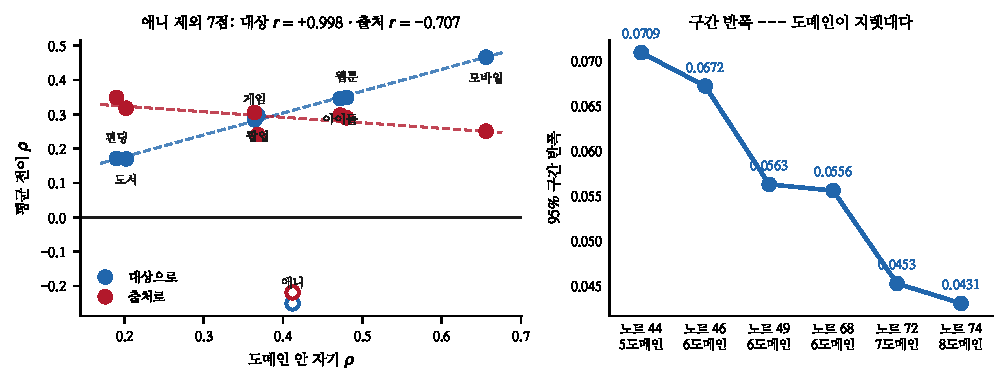
\includegraphics[width=\textwidth]{figs/eighth.pdf}
\caption{왼쪽 --- 자기 $\rho$와 전이(빈 표식이 애니). 오른쪽 --- 구간 반폭의 이력.}
\end{figure*}

\section{여덟째 도메인}

\begin{table}[t]
\centering\tsize
\caption{모바일 게임. 축 배선을 스팀 게임과 같게 맞췄다.}
\begin{tabular}{lll}
\toprule
슬롯 & 모바일 & 스팀 게임 \\
\midrule
라벨 & 평가 참여자 수 & 리뷰 총계 \\
타깃 폭 & 지원 언어 수 & 언어 수 \\
매장 노출도 & 개발사 이력 & 퍼블리셔 이력 \\
입장 허들 & 가격 & 가격 \\
굿즈 규모 & 앱 용량 & 설치 용량 \\
\midrule
표본 & 1,991건 & 472건 \\
\bottomrule
\end{tabular}
\end{table}

배선을 같게 맞춘 이유가 있다. 노트 51 · 52가 시장의 성질과 배선의 효과를 못
갈랐다. 배선이 같으면 \textbf{두 도메인의 차이가 배선이 아니라 시장에서 온다}는
것이 보장된다. 표본은 앱스토어 게임 대분류와 하위 장르 열아홉, 무료/유료/매출
세 차트 각 100위 --- 스팀 도메인이 topsellers 를 쓴 것과 같은 방식이다.

\section{판정치가 올랐다}

\begin{table}[t]
\centering\tsize
\caption{여덟 도메인 8,171건 · 56셀.}
\begin{tabular}{lrrrr}
\toprule
도메인 & $n$ & 자기 $\rho$ & 앙상블 & 출처로 \\
\midrule
\textbf{모바일} & 1991 & \textbf{$+$0.656} & \textbf{$+$0.640} & $+$0.251 \\
웹툰 & 2817 & $+$0.480 & $+$0.481 & $+$0.290 \\
팝업 & 75 & $+$0.368 & $+$0.452 & $+$0.241 \\
아이돌 & 62 & $+$0.472 & $+$0.439 & $+$0.298 \\
게임 & 472 & $+$0.364 & $+$0.386 & $+$0.305 \\
도서 & 242 & $+$0.202 & $+$0.238 & $+$0.318 \\
펀딩 & 400 & $+$0.190 & $+$0.211 & \textbf{$+$0.349} \\
애니 & 1419 & $+$0.412 & $-$0.258 & $-$0.219 \\
\midrule
\multicolumn{2}{l}{앙상블 판정치} & \multicolumn{2}{r}{\textbf{$+$0.3235}} &
$[+0.274, +0.360]$ \\
\multicolumn{2}{l}{셀 평균} & \multicolumn{2}{r}{$+$0.2291} &
$[+0.179, +0.258]$ \\
\bottomrule
\end{tabular}
\end{table}

$+$0.2744에서 $+$0.3235다. 반폭은 0.0453에서 0.0431로, 노트 69가 예측한
$\sqrt{42/56}$(0.039)보다는 덜 줄었다.

\section{법칙이 완성됐다}

\begin{table}[t]
\centering\tsize
\caption{자기 $\rho$와 전이의 상관.}
\begin{tabular}{lrr}
\toprule
& 대상으로 & 출처로 \\
\midrule
여덟 도메인 전부 & $+$0.401 & $-$0.182 \\
\textbf{애니 제외 일곱} & \textbf{$+$0.998} & $-$0.707 \\
\bottomrule
\end{tabular}
\end{table}

\claimx{도메인의 대상 전이 성적은 그 도메인의 \emph{자기} 상관으로 거의 완전히
결정된다 --- 일곱 점에서 $r=+0.998$이다. 노트 33 · 37의 ``전이 천장은 대상의
인자 공간 자기 상관''이 여덟 도메인에서 확증된다.}{애니를 뺀 상관이다. 애니를
넣으면 $+$0.401이다 --- 방향이 뒤집힌 도메인은 법칙 밖에 있다.}

$r=+0.998$이 일곱 점이라는 것을 감안해야 한다. 그래도 이 프로젝트에서 나온
가장 강한 규칙성이고, 실용적 함의가 분명하다.

\begin{quote}\fontsize{9.5}{11.5}\selectfont
\textbf{새 도메인이 대상으로 얼마나 좋을지는 그 도메인만 보고 안다.} 전이를
재려면 다른 일곱 도메인이 필요한데, 자기 상관은 그 도메인 하나로 잰다.
\emph{어느 카테고리를 다음에 붙일지 고르는 데 쓸 수 있다.}
\end{quote}

\section{가장 잘 맞히는 것이 가장 못 가르친다}

\begin{table}[t]
\centering\tsize
\caption{팝업을 맞히는 출처들.}
\begin{tabular}{lrr}
\toprule
출처 & $\rho$ & 자기 $\rho$ \\
\midrule
게임 & \textbf{$+$0.445} & $+$0.364 \\
아이돌 & $+$0.476 & $+$0.472 \\
펀딩 & $+$0.473 & $+$0.190 \\
도서 & $+$0.450 & $+$0.202 \\
웹툰 & $+$0.324 & $+$0.480 \\
\textbf{모바일} & \textbf{$+$0.223} & \textbf{$+$0.656} \\
애니 & $-$0.310 & $+$0.412 \\
\bottomrule
\end{tabular}
\end{table}

모바일은 자기 도메인을 가장 잘 설명하는데 팝업에는 가장 못 옮긴다(양수 중
최저). 나머지 평균 $+$0.434보다 0.211 낮다. \textbf{자기 라벨에 잘 맞는 축을
고를수록 그 축은 다른 데로 못 간다} --- 노트 40이 처음 적고 노트 51 · 68이
확인한 것의 가장 극단적인 사례다.

\section{닮은 것이 특별하지 않다}

\begin{table}[t]
\centering\tsize
\caption{표면이 거의 같은 두 도메인. 애니 제외 평균과 비교.}
\begin{tabular}{lrrr}
\toprule
셀 & $\rho$ & 나머지 평균 & 차이 \\
\midrule
게임 $\to$ 모바일 & $+$0.601 & $+$0.548 & $+$0.052 \\
모바일 $\to$ 게임 & $+$0.364 & $+$0.387 & $-$0.023 \\
\midrule
게임 $\to$ 팝업 & $+$0.445 & $+$0.389 & $+$0.056 \\
모바일 $\to$ 팝업 & $+$0.223 & $+$0.434 & $-$0.211 \\
\bottomrule
\end{tabular}
\end{table}

\claimx{표면이 닮았다고 서로에게 특별히 좋은 출처가 되지 않는다. 스팀 게임과
모바일 게임은 라벨도 축도 거의 같은데 쌍 이점이 $+$0.052 / $-$0.023이다.
전이를 만드는 것은 표면 유사성이 아니라 자기 상관의 높낮이다.}{배선을 같게
맞춘 것이 오히려 이점을 지웠을 수 있다 --- 각자 최적 배선을 찾았다면 달랐을
것이다.}

\section{방향은 안 뒤집혔다}

여덟째 도메인이 노트 69 이후의 질문에 답한다 --- \textbf{두 번째 사례는 안
왔다.} 모바일의 세 공통 축은 전부 라벨과 양의 상관이고 전이도 전부 양수다.
애니가 여전히 여덟 중 유일하다.

\begin{table}[t]
\centering\tsize
\caption{합의 정향과 게이트. 둘 다 대상 라벨 0건.}
\begin{tabular}{lrl}
\toprule
& 판정치 & 균등 대비 \\
\midrule
균등 & $+$0.3235 & --- \\
합의 뒤집기 & $+$0.3184 & $-$0.0057 보류 \\
합의 클립 & $+$0.3235 & $-$0.0003 보류 \\
게이트 & $+$0.3234 & --- \\
\bottomrule
\end{tabular}
\end{table}

합의는 여덟 도메인에서도 애니를 정확히 지목한다(팝업 가중치에서 애니만
$-$0.86). 그런데 \textbf{이득이 0이 됐다} --- 노트 72의 희석이 도메인이 늘수록
강해져 일곱 중 하나가 되면 고칠 것이 거의 없다. 게이트는 노트 73에서 무너졌던
것이 이제 안 무너지지만(셀 42$\to$56) 균등과 같다.

\begin{quote}\fontsize{9.5}{11.5}\selectfont
\textbf{합치는 것 위로 더 얹을 것이 아직 없다.} 방향 교정도 학습된 가중치도
균등 앙상블을 못 이긴다. 도메인을 늘리는 것만 값을 한다.
\end{quote}

\section{한계}

\begin{itemize}[leftmargin=1.1em,itemsep=0.15em]
\item $r=+0.998$이 일곱 점이다. 여덟째 · 아홉째를 넣으면 내려갈 것이다.
\item 모바일 미디어 투입 축이 14\%만 관측돼(스크린샷 결측) 사실상 네 축이다.
\item 모바일 표본이 인기 차트라 롱테일이 없다. 스팀 도메인과 같은 한계다.
\item 앱 용량은 업데이트로 늘어난다 --- 스팀 설치 용량과 같은 약한 누적이다.
\item 반폭이 0.0453$\to$0.0431로 예측(0.039)만큼 안 줄었다. 모바일이 유난히
      큰 도메인이라 셀 수의 $n^{-1/2}$가 안 맞는 것으로 보이지만 확인 안 했다.
\item 팝업 앙상블이 $+$0.459에서 $+$0.452로 또 조금 내렸다. 노트 72와 같은
      상황이고 여전히 판정치와 제품 목표의 간극이다.
\end{itemize}

\section{다음}

\begin{enumerate}[leftmargin=1.3em,itemsep=0.15em]
\item \textbf{자기 상관으로 다음 도메인을 고른다.} $r=+0.998$이면 후보 도메인의
      자기 상관만 재서 넣을지 정할 수 있다 --- 수집 전에.
\item 팝업 앙상블이 두 번 연속 내렸다. 팝업만을 목표로 한 판정치를 만들어
      일곱 평균과 얼마나 갈리는지 본다.
\item 애니의 방향을 정본에서 고칠지 결정한다. 지금은 판정치를 $-$0.10쯤
      깎고 있고, 노트 70의 32건 규약을 적용하면 고칠 수 있다.
\item 아홉째 도메인 --- 셀 56$\to$72.
\end{enumerate}

\vspace{0.6em}
\hrule height 0.3pt
\vspace{0.5em}
{\footnotesize
\textbf{참고문헌}\\[0.3em]
Ben-David, S. et al. (2010). A theory of learning from different domains.
\emph{Machine Learning}, 79(1--2), 151--175.\\[0.15em]
Rosenstein, M. T. et al. (2005). To transfer or not to transfer.
\emph{NIPS Workshop on Inductive Transfer}.\\[0.15em]
Meredith, W. (1993). Measurement invariance, factor analysis and factorial
invariance. \emph{Psychometrika}, 58(4), 525--543.\\[0.15em]
Standley, T. et al. (2020). Which tasks should be learned together in multi-task
learning? \emph{ICML}, 9120--9132.\\[0.15em]
Zamir, A. R. et al. (2018). Taskonomy: disentangling task transfer learning.
\emph{CVPR}, 3712--3722.\\[0.15em]
Efron, B., Tibshirani, R. J. (1993). \emph{An Introduction to the Bootstrap}.
Chapman \& Hall.
}

\end{document}
